
%(BEGIN_QUESTION)
% Copyright 2006, Tony R. Kuphaldt, released under the Creative Commons Attribution License (v 1.0)
% This means you may do almost anything with this work of mine, so long as you give me proper credit

Skisser kvalitativt hvordan en regulator med {\it kun integralvirkning} responderer over tid på endringene i prosessvariabelen vist her:

$$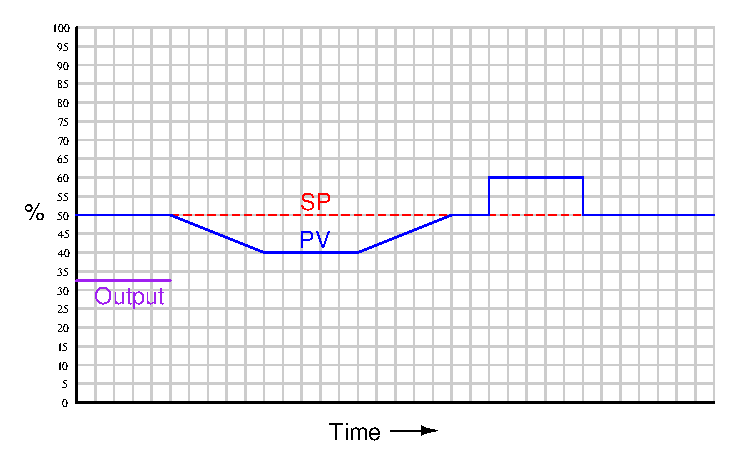
\includegraphics[width=15.5cm]{i01599x01.eps}$$

Anta {\it direkte} reguleringsvirkning.

\vskip 20pt \vbox{\hrule \hbox{\strut \vrule{} {\bf Forslag til sokratisk diskusjon} \vrule} \hrule}

\begin{itemize}
\item{} Finn en sikker metode for å plotte den krumme utgangsverdien til en integralregulator når den ``ser'' en rampende PV- eller SP-{\it inngangsverdi}.
\item{} Forklar hvordan utgangstrenden ville sett annerledes ut hvis tidsperioden for det andre avviket (der PV hopper bort fra og tilbake til SP i firkantsignal-form) var lengre.
\end{itemize}

\underbar{file i01599}
%(END_QUESTION)





%(BEGIN_ANSWER)

Regulatorutgangens graf vist her er kun {\it kvalitativ}. Selv om den er tegnet i riktig proporsjon (dvs. alle endringer i utgangen er riktig skalert relativt til hverandre), er selve skalaen vilkårlig og matcher derfor ikke nødvendigvis skalaen i din egen skisse:

$$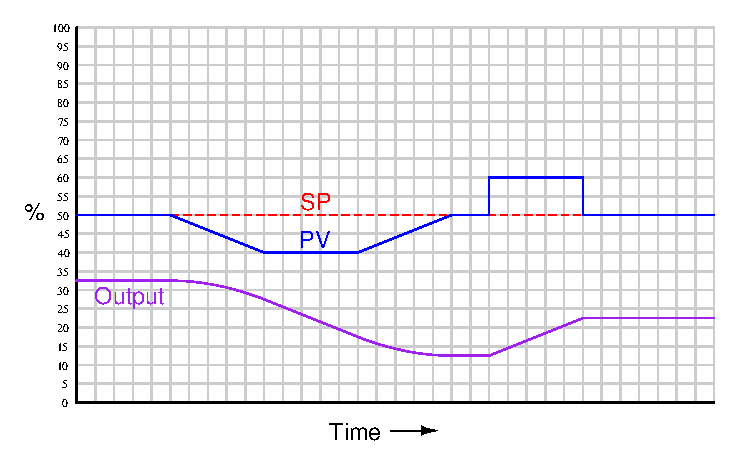
\includegraphics[width=15.5cm]{i01599x02.eps}$$

%(END_ANSWER)





%(BEGIN_NOTES)

$$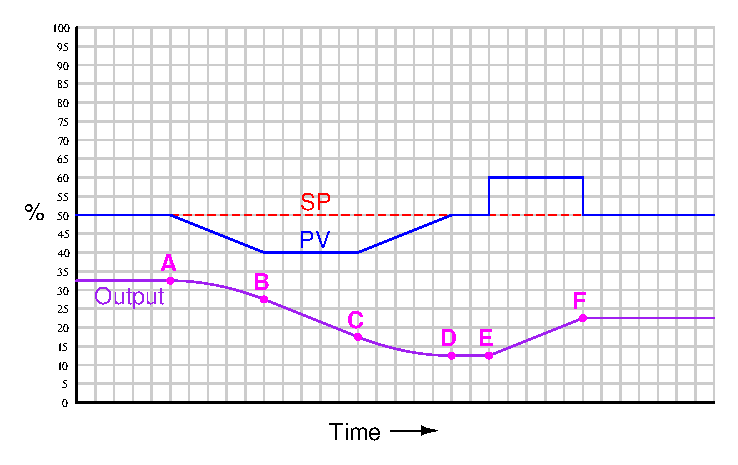
\includegraphics[width=15.5cm]{i01599x03.eps}$$

Utgangens endringsrate øker når avviket mellom PV og SP øker, noe som gir den nedoverkrummede utgangsresponsen fra punkt A til punkt B. Når PV flater ut mellom punkt B og C, holder utgangens endringsrate seg konstant, og da tegnes en rett linje nedover med samme stigning som kurven hadde ved punkt B. Mellom punkt C og D går PV tilbake mot SP til avviket blir null, og da flater utgangen ut etter hvert som stigningen går mot null.

Mellom punkt D og E holder utgangen posisjonen sin, fordi det ikke er noe avvik mellom PV og SP i dette tidsområdet. Når en plutselig ``trinnendring'' i PV skjer ved punkt E, integrerer utgangen med konstant hastighet oppover, og flater deretter ut når PV igjen blir lik SP.

%INDEX% Control, integral: graphing controller response

%(END_NOTES)
